\documentclass[letterpaper]{article}

\usepackage[top=1in, bottom=1in, left=1in, right=1in]{geometry}
\usepackage{float}
\usepackage{graphicx}
\usepackage{caption}
\usepackage{subcaption}
\usepackage{amsmath}
\usepackage{fancyhdr}
\setlength{\headheight}{15.2pt}

\pagestyle{fancy}
\lhead{Water Runner Simulation}
\lfoot{Nitish Thatte}
\cfoot{\thepage}
\rfoot{\today}

\title{Water Runner Simulation}
\author{Nitish Thatte}

\begin{document}
\maketitle

\section{Four Bar Angle Calculations}
\begin{figure}[htb]
	\centering
	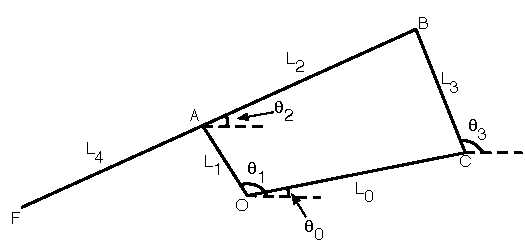
\includegraphics{4bar.pdf}
	\caption{Labeled 4-bar leg mechanism.}
	\label{fig:4bar}
\end{figure}
\subsection{Angular Position}
Under the assumption that $\theta_0 = 0$ and given $\theta_1$ angles $\theta_2$ and $\theta_3$ can be obtained as follows. First, we write the relationship between points $A$ and $B$ on the four bar linkage

\begin{equation}
	|B - A|^2 - L_2^2 = 0
	\label{eq:BArel}
\end{equation}

\begin{align}
	A &= \begin{pmatrix} L_1 \cos \theta_1 \\ L_1 \sin \theta_1 \end{pmatrix} \label{eq:Aloc}\\
	B &= \begin{pmatrix} L_0 \\ 0 \end{pmatrix} + \begin{pmatrix} L_3 \cos \theta_3 \\ L_3 \sin \theta_3 \end{pmatrix} \label{eq:Bloc}
\end{align}

\noindent Plugging equations \ref{eq:Aloc} and \ref{eq:Bloc} into \ref{eq:BArel} yields
\begin{align}
	0 &= (L_0 + L_3 \cos \theta_3 - L_1 \cos \theta_1)^2 + (L_3 \sin \theta_3 - L_1 \sin \theta_1)^2 - L_3^2 \notag \\
	  &= L_0^2 + 2 L_0 L_3 \cos \theta_3 - 2 L_0 L_1 \cos \theta_1 + L_3^2 \cos^2 \theta_3 - 2 L_3 L_1 \cos \theta_3 \cos \theta_1 \notag \\
	  & \quad + L_1^2 \cos \theta_1 + L_3^2 \sin^2 \theta_3 - 2 L_3 L_1 \sin \theta_3 \sin \theta_1 + L_1^2 \sin \theta_1^2 - L_2^2 \notag \\
	  &= (2 L_0 L_3 - 2 L_1 L_3 \cos \theta_1) \cos \theta_3 - 2 L_1 L_3 \sin \theta_1 \sin \theta_3 \notag\\
	  & \quad + L_3^2 + L_1^2 + L_0^2 - L_2^2 - 2L_0 L_1 \cos \theta_1
\end{align}

\noindent Grouping the terms that do not depend on $\theta_3$ 

\begin{align*}
	\alpha &= 2 L_0 L_3 - 2 L_1 L_3 \cos \theta_1 \\
	\beta &= -2 L_1 L_3 \sin \theta_1 \\
	\gamma &= L_1^2 L_3^2 L_0^2 - L_2^2 - 2 L_0 L_1 \cos \theta_1 
\end{align*}

\noindent If we define $\delta = \tan^{-1} \left( \frac{\beta}{\alpha} \right)$ then it follows that

\begin{equation*}
	\cos \delta \cos \theta_3 + \sin \delta \sin \theta_3 + \frac{\gamma}{\sqrt{\alpha^2 + \beta^2}} = 0
\end{equation*}

\noindent Therefore, 

\begin{align*}
	\theta_3 &= \delta \pm \cos^{-1} \left( \frac{- \gamma}{\sqrt{\alpha^2 + \beta^2}} \right) \\
	\theta_2 &= \tan^{-1} \left( \frac{ L_3 \sin \theta_3 - L_1 \sin \theta_1}{L_0 + L_3 \cos \theta_3 - L_1 \sin \theta_1} \right)
\end{align*}

\subsection{Angular Speed}

Loop closure requires that

\begin{align}
	A + (B - A) &= C + (C - B) \notag \\
	\dot{A} - \frac{d}{dt} (B - A) &= \frac{d}{dt} ( B - C) \label{eq:dloop}\\
	\begin{pmatrix} -L_1 \sin \theta_1 \\ L_1 \cos \theta_1 \end{pmatrix} \dot{\theta}_1 + \begin{pmatrix} -L_3 \sin \theta_3 \\ L_3 \cos \theta_3 \end{pmatrix} \dot{\theta}_3 &= \begin{pmatrix} -L_2 \sin \theta_2 \\ L_2 \cos \theta_2 \end{pmatrix} \dot{\theta}_1 \notag
	\end{align}

\noindent Rearranging terms yields a system of linear equations that allows us to solve for $\dot{\theta}_3$ and $\dot{\theta}_2$ given $\dot{\theta}_1$,

\begin{equation}
	\begin{pmatrix} -L_3 \sin \theta_3 && L_2 \sin \theta_2 \\ L_3 \cos \theta_3 && - L_2 \cos \theta_2 \end{pmatrix} \begin{pmatrix} \dot{\theta}_3 \\ \dot{\theta}_2 \end{pmatrix} = \begin{pmatrix} -L_1 \sin \theta_1 \\ L_1 \cos \theta_1 \end{pmatrix} \dot{\theta}_1
\end{equation}

\subsection{Angular Acceleration}

Differentiating the loop closure equation (\ref{eq:dloop}) yields:

\begin{equation}
	\ddot{A} + \frac{d^2}{dt^2} (B -A) = \frac{d^2}{dt^2} (B - C) \\
\end{equation}

\begin{equation*}
	\begin{pmatrix} - L_1 \sin \theta_1 \\ L_1 \cos \theta_1 \end{pmatrix} \ddot{\theta}_1 - \begin{pmatrix} L_1 \cos \theta_1 \\ L_1 \sin \theta_1 \end{pmatrix} \dot{\theta}_1^2 + \begin{pmatrix} - L_2 \sin \theta_2 \\ L_2 \cos \theta_2 \end{pmatrix} \ddot{\theta}_2 - \begin{pmatrix} L_2 \cos \theta_2 \\ L_2 \sin \theta_2 \end{pmatrix} \dot{\theta}_2^2 = \begin{pmatrix} - L_3 \sin \theta_3 \\ L_3 \cos \theta_3 \end{pmatrix} \ddot{\theta}_3 - \begin{pmatrix} L_3 \cos \theta_3 \\ L_3 \sin \theta_3 \end{pmatrix} \dot{\theta}_3
\end{equation*}

\noindent Rearranging terms yields a system of linear equations that allows us to solve for $\ddot{\theta}_3$ and $\ddot{\theta}_2$ given $\ddot{\theta}_1$, $\dot{\theta}_1$, $\dot{\theta}_2$, $\dot{\theta}_3$,

\begin{equation}
	\begin{pmatrix} -L_3 \sin \theta_3 && L_2 \sin \theta_2 \\ L_3 \cos \theta_3 && -L_2 \cos \theta_2 \end{pmatrix} \begin{pmatrix} \ddot{\theta}_3 \\ \ddot{\theta}_2 \end{pmatrix} = \begin{pmatrix} -L_1 \sin \theta_1 \\ L_1 \cos \theta_1 \end{pmatrix} \ddot{\theta}_1 - \begin{pmatrix} L_1 \cos \theta_1 \\ L_1 \sin \theta_1 \end{pmatrix} \dot{\theta}_1^2 - \begin{pmatrix} L_2 \cos \theta_2 \\ L_2 \sin \theta_2 \end{pmatrix} \dot{\theta}_2^2 + \begin{pmatrix} L_3 \cos \theta_3 \\ L_3 \sin \theta_3 \end{pmatrix} \dot{\theta}_3^2
\end{equation}
\end{document}
